%!TEX root = PhD_Thesis.tex
\chapter[Recursive Estimation of Needle Pose]{Recursive Estimation of Needle Pose for Ultrasound-Guided Needle Steering}

\section{Introduction}
Although ultrasound has many advantages as an imaging modality, it produces noisy data compared to CT or MR imaging. This is especially true when using high-frequency vibration and Doppler ultrasound imaging to segment a curved needle, as described in Chapter 2. While we demonstrated that this approach can reveal the curved shape of the needle, the resulting measurement error is large relative to the desired precision of percutaneous ablation. (Clinicians using medical image guidance systems can manually position needle tips within approximately 2~mm of a target in similar interventions~\cite{Crocetti2008}.) Manual localization of a steerable needle in ultrasound data, which is described in this chapter, also involves large amounts of measurement noise. A further difficulty is that ultrasound imaging provides infrequent measurements, as the result of the low volumetric framerate of 3D imaging. 

In this chapter, to attain clinically relevant targeting precision using sparse, noisy measurements, we describe a model-based recursive estimation scheme known as an unscented Kalman filter (UKF). This filter relies on experimental quantification of process and measurement noise for ultrasound-guided needle steering in biological tissue, which was performed using an electromagnetic tracking system as a reference.
 
This chapter is divided into two main sections. Section~\ref{sec:UKF} describes our UKF estimation scheme. Section~\ref{sec:AutonomousControl} describes validation of the scheme through closed-loop steering experiments in simulation and bench-top tissue models. The work described in this chapter was published in the proceedings of the IEEE/RSJ International Conference on Intelligent Robotics and Systems~\cite{Adebar2014a}.

%======================================================================
\section{Estimation Scheme}
%======================================================================
\label{sec:UKF}
\subsection{Needle Steering Model}
Our kinematic model of needle steering is based on the unicycle model of steerable needle motion~\cite{Park2005,Webster2006}; we assume the needle travels along curved path sections that are tangent to each other. To begin, we define the needle tip frame. As shown in Fig.~\ref{fig:NeedleKinematics}, this frame is attached to the tip of the steerable needle, and oriented so that its \textit{z}-axis is tangent to the needle at the tip, and its \textit{y}-axis points towards the center of curvature. In this model, the state of the needle is described by the pose of the needle tip frame relative to a reference frame, in our case the 3D ultrasound frame or robot frame. 

\subsubsection{Needle State Representation}
Needle tip position is represented by a vector ${p} \in \mathbb{R}^3$. There are several possible representations of tip orientation, including quaternions, Euler angles, and axis-angle rotation vectors. We have elected to use a rotation matrix ${R} \in \textrm{SO(3)}$. This is a singularity-free representation. To describe differential rotations, we will also frequently use the axis-angle rotation vector representation $r \in \textrm{so(3)}$, which can be calculated directly from ${R}$. The state ${x}$ is thus defined as
\begin{align}
{x} = \{p \in \mathbb{R}^3, R \in \textrm{SO(3)}\}
\end{align}

\begin{figure*}[!t]
\centering
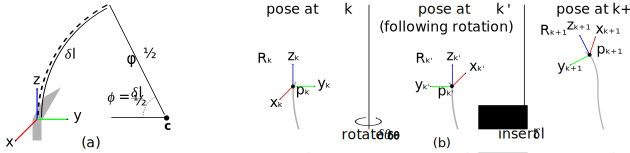
\includegraphics[width=\textwidth]{Images/Chapter4/NeedleKinematics/NeedleKinematics}%
\caption[Kinematic model of needle steering]{Kinematic model of needle steering~\cite{Webster2006} used in image-guided control: (a) Needle tip frame. The $z$-axis is tangent to the needle at the tip (ignoring the bevel or prebent section), the $y$-axis points towards the center of curvature. The needle path is an arc within the $y$-$z$ plane with radius $\rho$ and arc length $\delta l$. (b) Progression of the needle tip frame during steering. The steerable needle insertion is divided into increments, with incremental needle rotation angle ($\delta\theta$), incremental insertion distance ($\delta l$) and radius of curvature ($\rho$) updated as command inputs between increments. These command inputs define the transition of state vector ${x}$.}
\label{fig:NeedleKinematics}
\end{figure*}

\subsubsection{State Transition Model}
Based on the kinematic model of needle steering~\cite{Webster2006}, we define the transition of needle state to the next time interval, ${x_{k+1}}$, as a function of the current state, ${x_{k}}$, a vector of command inputs, ${u_{k}}$, and a vector of process noise, ${w}$:
\begin{align}
{x_{k+1}} = f({x_k}, {u_k}, {w}).
\end{align}
In our model, we divide needle steering into incremental insertions. Command inputs are applied between incremental insertions, and include change in needle base rotation $\delta\theta$, incremental insertion distance $\delta l$, and radius of incremental needle path $\rho$:
\begin{align}
{u} = \begin{bmatrix} \delta\theta & \delta l & \rho\end{bmatrix}^{\text{T}}.
\end{align}
The radius of the needle path can be experimentally measured as described in the previous chapters. The radius can also be adjusted using duty cycling~\cite{Minhas2007}, a control approach that uses short, variable periods of insertion with and without rotation to adjust needle curvature from maximum curvature to straight. System variability is modeled using nonadditive Gaussian noise in the state transition model. The noise ${w}$ can be separated into a position component, ${p_w} \in \mathbb{R}^3$, and an orientation component, ${R_w} \in SO(3)$. The index $k$ is omitted from the vector ${w}$ to signify the random nature of the vector.

The state transition function $f$ can be viewed as a transformation of the tip frame, as shown in Fig.~\ref{fig:NeedleKinematics}. The needle tip frame at time ${k}$ has pose defined by ${p_{k}}$ and ${R_{k}}$. The needle tip frame is first rotated about its $z$-axis by $\delta\theta$ to yield the rotated tip frame:
\begin{align}
{R_{k'}} = {R_{k}}{Rz}(\delta\theta).
\end{align}
The needle is then inserted a distance $\delta l$, with the tip following a circular path of radius $\rho$. From the definition of the tip frame shown in Fig.~\ref{fig:NeedleKinematics}, we know that the needle path will lie in the $y$-$z$ plane of the rotated frame defined by ${R_{k'}}$. The position of the needle tip after insertion relative to the rotated frame can be found directly from the geometry of the circular path:
\begin{align}
{^{k'}p_{k+1}} = \begin{bmatrix}0\\ \rho(1-\cos(\frac{\delta l}{\rho})) \\ \rho\sin(\frac{\delta l}{\rho})\end{bmatrix}.
\end{align}
Transforming this vector into the world frame, and including process noise yields an expression for $p_{k+1}$:
\begin{align}
{p_{k+1}} = {R_{k}}{Rz}(\delta\theta){^{k'}p_{k+1}}+{p_k} +{p_w}.
\end{align}
%\begin{align}
%\begin{array} {lcl} {p_{k+1}} & = & {R_{k}}{Rz}(\delta\theta){^{k'}p_{k+1}}+{p_k} +{p_w} \\ & = & {R_{k}}{Rz}(\delta\theta)\begin{bmatrix}0\\ \rho(1-\cos(\frac{l}{\rho})) \\ \rho\sin(\frac{l}{\rho})\end{bmatrix}+{p_k} +{p_w}.\end{array}
%\end{align}
The orientation of the tip frame after insertion can be defined using the same rotation matrices. Similar to other studies that have applied Kalman filters to orientation representations~\cite{Kraft2003}, we include orientation noise as an initial disturbance to the state vector, ${R_w}$.
The updated tip frame orientation is thus
\begin{align}
{R_{k+1}} = {R_{k}}{R_w}{Rz}(\delta\theta){Rx}\left(\begin{matrix}-\frac{\delta l}{\rho}\end{matrix}\right).
\end{align}
The vector ${r_{k+1}}$ is the rotation vector equivalent of ${R_{k+1}}$.

\subsubsection{Measurement Model}
Based on our 3D ultrasound needle segmentation method~\cite{Adebar2013}, we define the measurement model as full-state feedback with additive measurement noise vector ${v}$:
\begin{align}
{z_{k}} = {x_k} + {v}.
\end{align}
This model assumes that the automatic or manual segmentation method can measure the full 6DOF pose of the needle tip frame. Although rotation around the axis of a needle can not generally be resolved by 3D ultrasound, in the case of a curved steerable needle we can use the direction of needle curvature to estimate the $y$-axis of the needle frame.

\subsection{Unscented Kalman Filter}
The unscented Kalman Filter is an extension of the classical Kalman filter to nonlinear systems, and uses a set of sampled points around a mean value to represent distributions~\cite{Julier1997}. For brevity, we omit a detailed description of the typical UKF, and refer the reader to~\cite{Thrun2005} for a complete explanation. Our implementation of the UKF follows the original description of the algorithm~\cite{Julier1997}, with several modifications as described below. 

\subsubsection{Calculation of the Mean}
The first modification is our method for calculating the mean $\overline{x}$ of a set of states $x_0 \dots x_k$. In the UKF, this method is used to recover the mean and covariance of the state estimate from a set of transformed sigma points. Normally in a UKF, the state exists in a vector space, and can be represented by a vector $x \in R^n$. The mean of a set of vector states can be calculated as the sum of the states divided by the size of the set,
\begin{align}
\overline{x} = \frac{1}{k}\sum\limits_{i=1}^{k} x_i,
\end{align}
\noindent 
while the corresponding covariance can be calculated as:
\begin{align}
P = \frac{1}{k}\sum\limits_{i=1}^{k} (x_i-\overline{x})(x_i-\overline{x})^T.
\end{align}
\noindent
Our state includes the 3D position of the needle tip, represented by a vector ${p} \in \mathbb{R}^3$, and the 3D orientation of the needle tip, represented by a matrix ${R} \in \textrm{SO(3)}$. Because orientation is periodic, it is not possible to calculate the mean state or covariance using the above formulae. Instead, we use the iterative gradient descent approach proposed by Kraft~\cite{Kraft2003}. 

Given a set of state measurements $x_0 \dots x_k$, with each $x_i = \{p_i,R_i\}$, we calculate the mean position as:
\begin{align}
\overline{p} = \frac{1}{k}\sum\limits_{i=1}^{k} p_i.
\end{align}
We then calculate the set of equivalent axis-angle rotation vector representations $r_i \dots r_k$. To begin the gradient descent, we initialize the mean orientation estimate as $\overline{r} = r_0$. We define an orientation error in rotation matrix form as $E_i = R_i\overline{R}$, where $\overline{R}$ is again the equivalent rotation matrix representation of vector $\overline{r}$. Calculating this error for each of the $k$ orientations, we can form a measure of the difference between the current mean orientation estimate and the true mean orientation,
\begin{align}
\overline{e} = \frac{1}{k}\sum\limits_{i=1}^{k} e_i,
\end{align}
Since $\overline{e}$ is a rotation vector that points in the direction of the true mean orientation. The mean is then updated,
\begin{align}
\overline{R} = \overline{E} \overline{R}.
\end{align}
This correction is repeated until the norm of the adjustment vector $\overline{e}$ drops below an acceptable threshold ($1\times10^{-5}$ in our implementation).

\subsubsection{Calculation of the Covariance}
Calculating the covariance $P$ of a set of states $x_0 \dots x_k$ is straightforward after calculating the mean position and orientation as described. Comparing each state $x_i$ with the mean, we combine the position error with the calculated orientation error vector, to define a difference vector,
\begin{align}
d_i = \begin{bmatrix} p_i - \overline{p}\\ 
e_i
\end{bmatrix}.
\end{align}
The covariance $P$ can then be calculated directly as
\begin{align}
P = \frac{1}{k}\sum\limits_{i=1}^{k}dd^T.
\end{align}

\subsubsection{Injection of Process and Measurement Noise}
Since the effect of process noise on the state transition is nonadditive, we include the noise covariance matrices $Q$ and $R$ in the generation of the Sigma points. In other words, given a state estimate $\tilde{x} \sim N\left(\mu,P\right)$, we draw Sigma points from the distribution $\sim N\left(\mu,P+Q\right)$, and pass them through the state transition function.
 
%======================================================================
\section{Experimental Validation}
%======================================================================
\label{sec:AutonomousControl}
Application of the UKF requires an understanding of the relative amounts of uncertainty (\textit{i.e.}, noise) in the evolution of the state (process noise) and the measurement of the state (measurement noise). To quantify the process and measurement noise involved in 3D-ultrasound-guided needle steering, we first performed experimental measurements using samples of \textit{ex vivo} porcine liver tissue. We then validated our estimation scheme in simulated needle steering trials, and in bench-top needle steering experiments using the needle steering robot described in Chapter~2.

\subsection{Experimental Methods}
\subsubsection{Quantification of Process and Measurement Noise}
Process noise was quantified by using a magnetic tracking system to precisely measure the motion of a steerable needle tip during incremental insertion along constant curvature paths. A hollow steerable needle 0.80 mm in diameter was connected to the needle steering robot described in Chapter 2, and a 6DOF sensor attached to a magnetic tracking system (driveBAY; Ascension Technology Corp., Milton, VT) was inserted into the needle tip. The pose of the needle tip after each incremental step was compared with what was expected based on the previous pose and the process model. Denoting the state vector measured by the magnetic tracking system as $\hat{{x}}$, we determined an error vector ${w}$ at each step such that
\begin{align}
{\hat{x}_{k+1}} = f({\hat{x}_{k}}, {u_{\text{est}}}, {w}).
\end{align}
During these experiments, input vector ${u_{\text{est}}}$ was held constant at $[0, \text{3 mm}, \rho_{\text{est}}]^{T}$. The needle was inserted along four paths, with between fifteen and twenty measured positions per path. Initial tip frame orientation was measured by fitting a circular arc to the set of measured positions, and identifying the vectors tangent ($z$-axis) and normal ($x$-axis) to the arc at the initial tip position. Data analysis was performed offline using Matlab. 

The tip position measurements could be used directly, however the tip orientation measurements had to first be adjusted to conform to the definition of the needle tip frame given above. Specifically, the measured z-axis was aligned with the needle axis, but the measured x-axis and y-axis were not. To correct the orientation, a circular arc was fit to the measured tip points from each insertion, yielding an estimated radius of curvature $\rho_{est}$. The mean difference between the measured x-axes and the normal to the circular arc was used to correct the orientation measurements to be consistent with the needle tip frame.

Measurement noise was quantified by comparing automatic segmentation results from repeated 3D ultrasound scans of steerable needles in biological tissue. Between five and eleven repeated scans were performed for each of six needle tip poses. The needles were automatically segmented from each scan using the previously Doppler method described in Chapter 2. Data analysis was again performed offline in Matlab.

\subsubsection{Ultrasound-Guided Needle Steering Simulations}
We first evaluated our UKF algorithm in a series of simulated closed-loop needle steering trials. These simulations allowed us to compare our UKF results with the true needle tip state, which was not possible in the experiments described in the next section. In each trial, a target tip position and initial tip pose were identified in the 3D ultrasound coordinate system, and the needle tip was steered towards the target along a 3D path. Four initial scans were simulated to allow the UKF estimate to converge. Afterwards, the needle was steered in constant 3-mm incremental insertions using the UKF-filtered segmentation results to correct the needle rotation and path radius settings at each step. To provide a comparison baseline, each trial was also repeated using the unfiltered segmentation results as control feedback. 

The target point ${t}$ was varied according to a uniform distribution:
\begin{align}
{t} \sim U\left(
\begin{bmatrix} -20\\ 35\\ 30 \end{bmatrix},
\begin{bmatrix} 20\\ 65\\ 60 \end{bmatrix} \right).
\end{align}
Initial needle tip position was held constant: 
\begin{align*}
{p_{\text{init}}} = \begin{bmatrix} 0 & 50 & -40 \end{bmatrix}^{\text{T}}.
\end{align*}
Initial needle tip orientation was varied according to a normal distribution:
\begin{align}
{r_{\text{init}}} \sim N\left(
\begin{bmatrix} 0\\ 0\\ 0 \end{bmatrix},
\begin{bmatrix} 32.82 & 0 & 0\\ 0 & 32.82 & 0\\ 0 & 0 & 32.82 \end{bmatrix} \right).
\end{align}
Simulations were implemented in Matlab.

\subsubsection{Ultrasound-Guided Needle Steering Experiments}
In addition to simulation tests, we performed a series of closed-loop needle steering experiments. The robot steered a 0.58 mm needle with a bevel tip in \textit{ex vivo} porcine liver tissue under 3D ultrasound guidance. The UKF algorithm was implemented in C++ and combined with algorithms for Doppler image segmentation. A SonixMDP ultrasound console (Ultrasonix Medical Corp., Richmond, Canada) with a convex mechanical 3D transducer (4DC7-3/40) was used for imaging. Similar to the simulated trials, a target was defined in the 3D ultrasound coordinate system and the needle was steered in constant 5-mm incremental insertions using sensor feedback to correct the needle rotation and path radius settings at each step. For comparison, six steering tests each were performed with and without the UKF.

\subsection{Results}
\subsubsection{Quantification of Process and Measurement Noise}
Across 66 samples of process noise, the mean position error (in millimeters) and mean orientation error (in degrees) were \[{\overline{p}_{w}} = \begin{bmatrix} 0.38 &-0.09 &0.17 \end{bmatrix}^{\text{T}}, {\overline{r}_{w}} = \begin{bmatrix} 0.43 &0.02 &0.50 \end{bmatrix}^{\text{T}}.\] To find the best-fit zero-mean Gaussian distribution to the process noise, we reflected the measured noise vectors, resulting in a sample covariance of
\begin{align*}
{\hat{Q}} = \begin{bmatrix} 
\phantom{-}0.39 	& -0.06 	& \phantom{-}0.15 		& \phantom{-}0.24 		& -0.05 	& \phantom{-}0.08\\ 
-0.06 			& \phantom{-}0.21  	& -0.10   	& -0.17 	& \phantom{-}0.17 		& -0.05\\
\phantom{-}0.15 	& -0.10 	& \phantom{-}0.16    	& \phantom{-}0.09 		& -0.08 	& \phantom{-}0.23\\
\phantom{-}0.24 	& -0.17 	& \phantom{-}0.09  	& \phantom{-}0.65 		& -0.34 	& -0.09\\
-0.05 	& \phantom{-}0.17		& -0.08 	& -0.34 	& \phantom{-}1.22		& \phantom{-}0.00\\
\phantom{-}0.08 	& \phantom{-}0.05		& \phantom{-}0.23  	& -0.09 	& \phantom{-}0.00 	& \phantom{-}2.49\\
\end{bmatrix}.
\end{align*}

In the measurement noise experiment, we assumed the mean of repeated segmentations at each tip pose was the true needle pose. This was necessary because we did not have a reference segmentation method for comparison (thin steerable needles are not generally visible in B-mode ultrasound). Across 60 observations of measurement noise, the sample covariance was
\begin{align*}
{\hat{R}} = \begin{bmatrix} 
\phantom{-}0.81 & \phantom{-}0.09 & -0.27 & \phantom{-}3.41 & \phantom{-}37.1 & \phantom{-}18.2\\ 
\phantom{-}0.09 & \phantom{-}1.10 & \phantom{-}0.51 & -17.7 & \phantom{-}20.2 & \phantom{-}4.97\\
-0.27 & \phantom{-}0.51 & \phantom{-}0.90 & -13.5 & \phantom{-}1.54 & -3.68\\
\phantom{-}3.41 & -17.7 & -13.5 & \phantom{-}3930 & -1720 & -375\\ 
\phantom{-}37.1 & \phantom{-}20.2 & \phantom{-}1.54 & -1720 & \phantom{-}7520 & \phantom{-}2740\\ 
\phantom{-}18.2 & \phantom{-}4.97 & -3.68 & -375 & \phantom{-}2740 & \phantom{-}1240\\
\end{bmatrix}.
\end{align*}
These experimental results give an indication of the relative levels of process and measurement noise, which is valuable for a Kalman filter formulation; however, only a relatively small number of measurements were practical for both experiments, and as a result it is difficult to infer characteristics of the underlying distributions. On the other hand, the process noise measurements, which were correlated and had non-zero mean, suggest that the kinematic model of needle steering we applied may not completely capture needle behavior in \textit{ex vivo} liver. While a more sophisticated bicycle model of needle kinematics exists~\cite{Webster2006}, it is identical to the unicycle model except when rotating the needle, which we did not do in our process noise experiments. With a more accurate kinematic model, we would expect the process noise to approximately follow a normal distribution with zero mean. This process noise would describe small deflections of the needle tip off the expected trajectory that would result from steering in an inhomogeneous biological material. The difference in the experimental measurements suggests further investigation is warranted.  

\begin{figure}[!t]
\centering
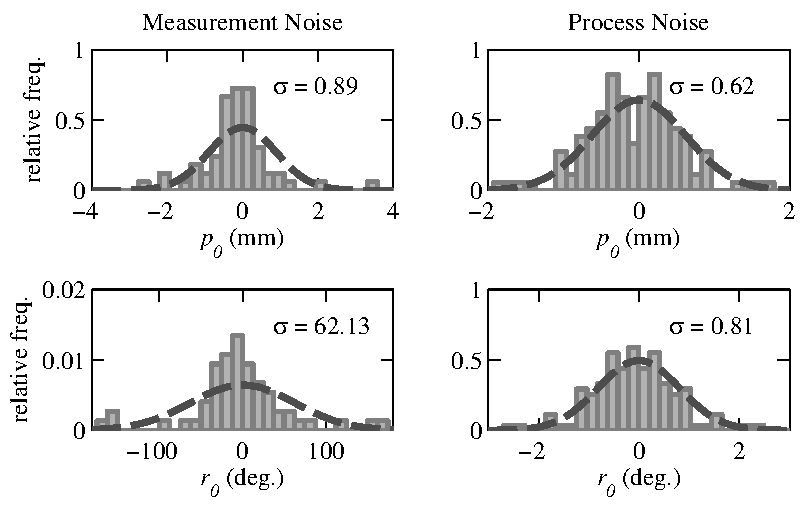
\includegraphics[width=0.75\columnwidth]{Images/Chapter4/Noise/Noise}%
\caption[Distributions of process and measurement noise]{Distributions of process and measurement noise for $p_0$ and $r_0$ components of position and orientation. Histograms of experimentally measured error vectors (gray bars) are compared with the normal distributions used in needle steering simulations.}
\label{fig:Noise}
\end{figure}

To make our simulations realistic, we chose to formulate the Kalman gains in the UKF without exact knowledge of the process or measurement noise distributions. Specifically, the UKF assumed both process and observation noise were uncorrelated and normally distributed with zero mean and variances of 
\begin{align*}
{Q} = \text{diag}(\begin{bmatrix} 0.2 & 0.2 & 0.2 & 3.28 & 3.28 & 3.28 \end{bmatrix}^{\text{T}}),
\end{align*}
\begin{align*}
{R} = \text{diag}(\begin{bmatrix} 1 & 1 & 1 & 3282 & 3282 & 3282 \end{bmatrix}^{\text{T}}).
\end{align*}

\subsubsection{3D-Ultrasound-Guided Needle Steering Simulations}
Over 10,000 simulation trials, the average error (mean~$\pm$~standard deviation) in final tip placement was 2.26~$\pm$~1.30~mm using the UKF-filtered segmentation results for feedback, and 11.85~$\pm$~7.36~mm using the unfiltered segmentation results. Based on a bootstrapped statistical test, the UKF resulted in a statistically significant increase in placement accuracy ($p~<~0.01$).

\begin{figure}[!h]
\centering
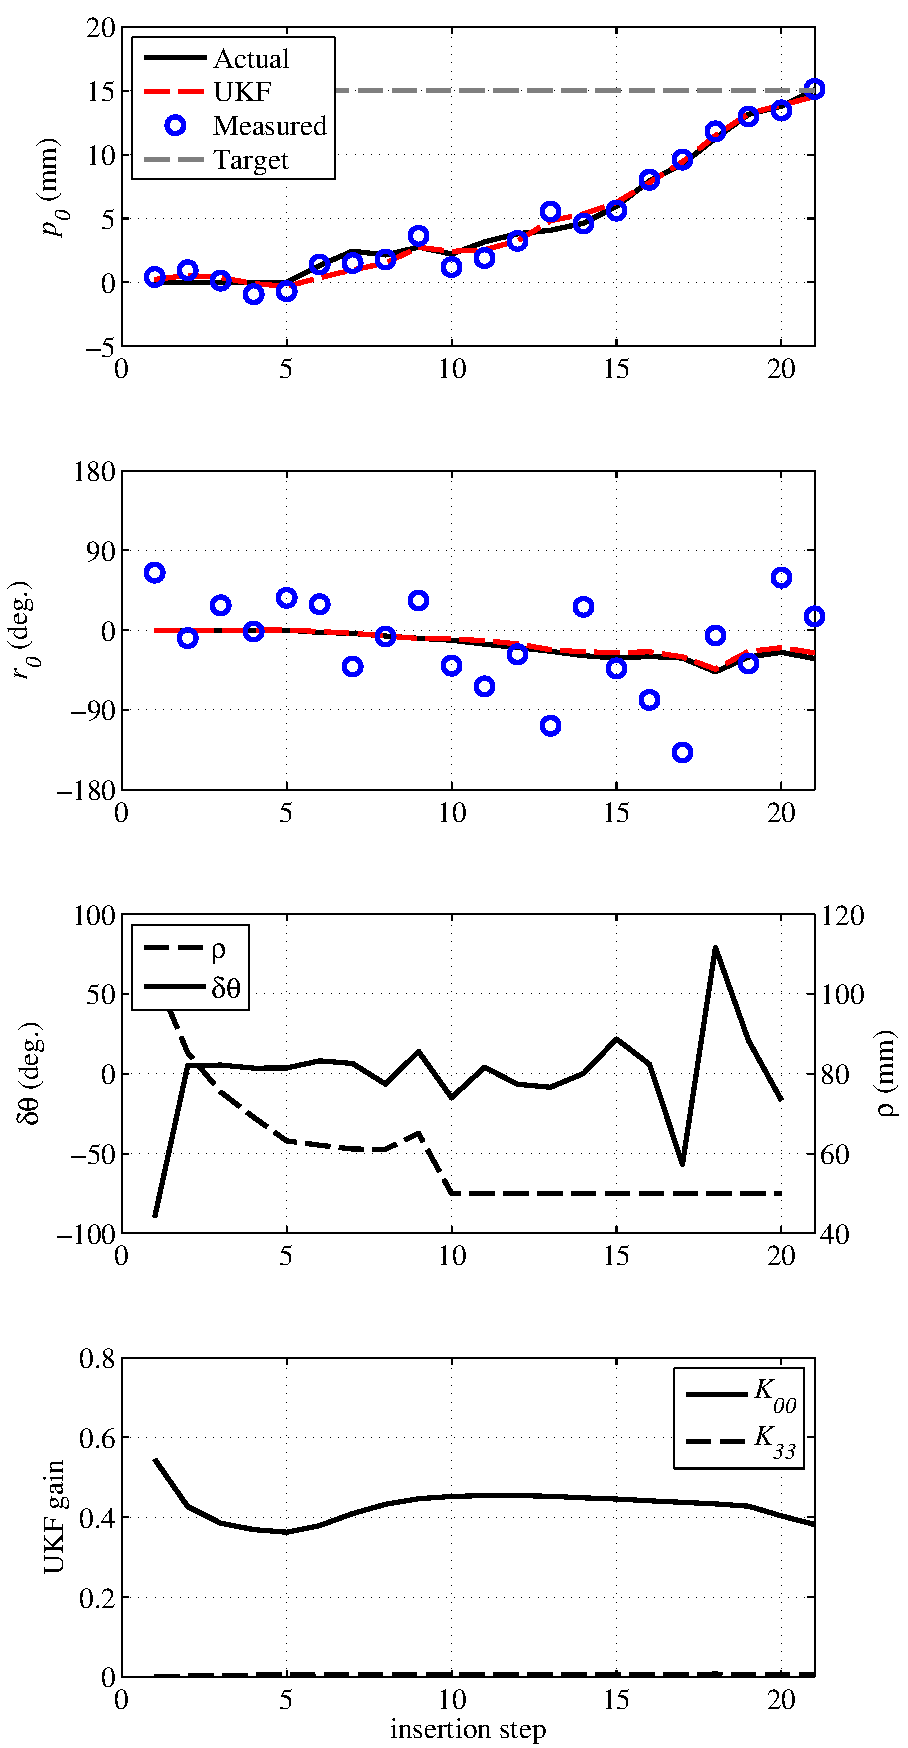
\includegraphics[width=0.5\columnwidth]{Images/Chapter4/SimulationResults/SimulationResults}%
\caption[Closed-loop needle steering results]{Closed-loop needle steering results. Actual, measured and UKF-estimated state vector elements $p_0$ and $r_0$ are shown for steering towards a target located at $p_0 = 15$. The resulting values of control variables $\delta\theta$ and $\rho$ are also plotted, and represent the control effort needed to overcome process variability inherent to steering in biological tissue. UKF gain values $K_{00}$ and $K_{33}$ show significant reliance on measured needle position, but relatively little reliance on measured needle orientation when forming the UKF estimate. }
\label{fig:SimulationResults}
\end{figure}   

Fig.~\ref{fig:Noise} shows experimental histograms of process and measurement noise for the first components of position and orientation (\textit{i.e.}, $p_0$ and $r_0$) compared to normal distributions with the same variance. In our needle steering simulations, we modeled the process and measurement noise as normally distributed, with zero mean and covariance equal to ${\hat{Q}}$ and ${\hat{R}}$ as defined above.

\begin{figure}[!t]
\centering
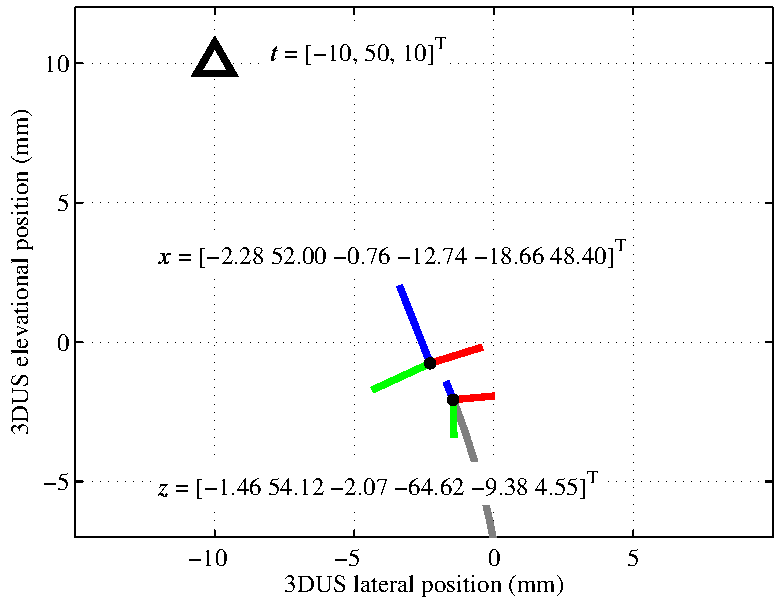
\includegraphics[width=0.7\columnwidth]{Images/Chapter4/ExperimentalResults/ExperimentalResults}%
\caption[Results using UKF in autonomous control]{Experimental results for closed-loop needle steering in \textit{ex vivo} porcine liver tissue. After seven iterations, the UKF estimate of needle pose ${x}$ (large axes) has less error in orientation than the measured needle pose ${z}$ (small axes), which is based entirely on the segmented needle curve (solid line). The robot continued steering towards the target point ${t}$, and achieved final placement error of 2.67 mm.}
\label{fig:ExperimentalResults}
\end{figure}

Fig.~\ref{fig:SimulationResults} shows simulation results from using the UKF-filtered segmentation data in closed-loop steering towards a target. The figure shows actual, measured and estimated values for two state elements (again $p_0$ and $r_0$), along with resulting control inputs ($\delta\theta$ and $\rho$) and UKF gains. In this simulation, the needle tip was steered from a point with $p_0 = 0$ towards a point at $p_0 = 15$. As seen in the figure, the UKF approach accurately estimated the true position and orientation despite large amounts of measurement noise, particularly in orientation. As mentioned above, the segmentation method we apply is based on measuring the centroid of irregular Doppler patches around the needle, and gives a relatively poor indication of needle tip orientation. The UKF estimate of tip orientation was thus based almost entirely on our kinematic model of needle steering, whereas the UKF estimate of tip position was based on both the kinematic model and the segmentation results. This is shown by the UKF gains $K_{00}$ and $K_{33}$, which represent how heavily measurements $z_0$ and $z_3$ are weighted versus the corresponding process model outputs at each iteration. As shown by the control inputs, the robot made a large initial rotation to steer the needle towards the target, then made small corrections as a result of the steering variability (process noise). Once the needle approached the target, larger rotations and tighter path radii were necessary to correct for variations. At the end of the trial the needle tip was 0.83 mm from the target.    

\subsubsection{3D-Ultrasound-Guided Needle Steering Experiments}
Table~\ref{table:Targeting Results} lists final tip placement error for each closed-loop steering test. Over six tests using the UKF, the average error was 2.69 mm. This is within one standard deviation of the mean simulation result, and approaches an acceptable error for clinical applications. Over six tests without the UKF, the average error was 11.39 mm, which is also within one standard deviation of the mean simulation result. The robot executed between nine and twelve incremental insertions in each test. 

\begin{table}[!h]
% increase table row spacing, adjust to taste
\renewcommand{\arraystretch}{1.3}
\centering
\caption{Tip placement errors in needle steering experiments}
\label{table:Targeting Results}
% Some packages, such as MDW tools, offer better commands for making tables
% than the plain LaTeX2e tabular which is used here.
\begin{tabulary}{\columnwidth}{| l | C | C | C | C | C | C | C |}
\hline
Test & 1 & 2 & 3 & 4 & 5 & 6 & avg. \\
\hline
UKF (mm) & 2.67 & 2.34 & 3.83 & 3.44 & 2.90 & 0.98 & 2.69 \\
\hline
No UKF (mm) & 9.89 & 13.41 & 9.03 & 11.12 & 10.14 & 14.74 & 11.39 \\
\hline
\end{tabulary}
\end{table}

Fig.~\ref{fig:ExperimentalResults} shows results from Test 1 with the UKF. In this test, the needle tip was intially located at ${p}~=~\begin{bmatrix} -0.80 & 53.26 & -14.04 \end{bmatrix}^{\text{T}}$ mm, and was steered towards the target at ${t} = \begin{bmatrix} -10 & 50 & 10 \end{bmatrix}^{\text{T}}$ mm. The figure shows the segmented needle curve, measured tip frame, and UKF-estimated tip frame after seven UKF iterations (four initial scans and three incremental insertions). At this point the UKF-estimated tip position was close to the measured tip position; however, the UKF-estimated tip orientation was significantly different from the measured tip orientation. This example illustrates the importance of the UKF in closed-loop robot control, since using the segmentation results directly would have caused the robot to falsely correct the needle orientation with a large rotation.     


